\documentclass[journal,12pt,twocolumn]{IEEEtran}
\usepackage{cite}
\usepackage{amsmath,amssymb,amsfonts,amsthm}
\usepackage{algorithmic}
\usepackage{graphicx}
\usepackage{textcomp}
\usepackage{xcolor}
\usepackage{txfonts}
\usepackage{listings}
\usepackage{enumitem}
\usepackage{mathtools}
\usepackage{gensymb}
\usepackage{comment}
\usepackage[breaklinks=true]{hyperref}
\usepackage{tkz-euclide}
\usepackage{braket}
\def\inputGnumericTable{}
\usepackage[latin1]{inputenc}
\usepackage{color}
\usepackage{array}
\usepackage{longtable}
\usepackage{calc}
\usepackage{multirow}
\usepackage{hhline}
\usepackage{ifthen}
\usepackage{lscape}
\usepackage{gvv} 
\usepackage{circuitikz}

\newtheorem{theorem}{Theorem}[section]
\newtheorem{problem}{Problem}
\newtheorem{proposition}{Proposition}[section]
\newtheorem{lemma}{Lemma}[section]
\newtheorem{corollary}[theorem]{Corollary}
\newtheorem{example}{Example}[section]
\newtheorem{definition}[problem]{Definition}
\newcommand{\BEQA}{\begin{eqnarray}}
\newcommand{\EEQA}{\end{eqnarray}}
\newcommand{\define}{\stackrel{\triangle}{=}}
\theoremstyle{remark}
\newtheorem{rem}{Remark}

\begin{document}

\bibliographystyle{IEEEtran}
\vspace{3cm}

\title{GATE 2022 IN-56}
\author{EE23BTECH11201 - Abburi Tanusha$^{*}$% <-this % stops a space
}
\maketitle
\newpage
\bigskip

\renewcommand{\thefigure}{\theenumi}
\renewcommand{\thetable}{\theenumi}

\vspace{3cm}

\maketitle
\textbf{Question:} 
The circuit shown is driven by a sinusoidal input voltage, $V_{\text{in}}$, resulting in the output voltage $V_{\text{out}}$. The frequency (in kilohertz) at which the voltage gain is 0 dB is (rounded off to two decimal places).
\begin{figure}[htb]
	\centering
	

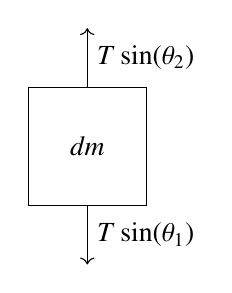
\begin{tikzpicture}[scale=0.75] % Adjust the scale factor as needed
    % Draw the square body
    \draw (0,0) rectangle node[pos=0.5] {$dm$} (2,2);
    
    % Add upward force T*sin(theta2)
    \draw[->, black] (1,2) -- node[right] {$T \sin(\theta_2)$} (1,3);
    
    % Add downward force T*sin(theta1)
    \draw[->, black] (1,0) -- node[right] {$T \sin(\theta_1)$} (1,-1);
\end{tikzpicture}




	\label{fig:1}
\end{figure}
\hfill(GATE IN 2022)\\
\textbf{Solution:} 
This circuit is an inverting OP-AMP. The transfer function of an inverting OP-AMP is given by\\
\begin{table}[h]
 	\centering
 	\resizebox{12 cm}{!}{
 		\begin{table}[H]
    \centering
    \renewcommand\thetable{1}
    \setlength{\extrarowheight}{9pt}
    \resizebox{0.51\textwidth}{!}{
    \begin{tabular}{|c|c|c|}
    \hline
    \textbf{$r\brak{i}$} & \textbf{$p\brak{i}$} & \textbf{$k\brak{i}$} \\ \hline
    $0.06029142-0.14682007jj$ &0.88475217+0.0445749j&$2.19006287\times10^{-5}$  \\ \hline
    $0.06029142+0.14682007jj$ &0.88475217-0.0445749j&$-$  \\ \hline
    $-0.06029459+0.02518904j$ &0.94427798+0.11485352jj&$-$  \\ \hline
    $-0.06029459-0.02518904j$ & 0.94427798-0.11485352j&$-$  \\ \hline
    \end{tabular}}
    \caption{Values of $ r(i) , p(i) , k(i)$}
    \label{tab:values of r(i) , p(i) , k(i)}
    \end{table}

 	}
 	\vspace{6 pt}
 	\caption{Parameters}
 	\label{tab:anu_label} 
 \end{table}
\begin{align}
Z_1 &= R_1 \\
Z_2 &= \frac{R_2}{1+j \omega R_2C} \\
\frac{1}{Z_2} &= \frac{1}{R_2} + j\omega C \\
\frac{V_{\text{out}}}{V_{\text{in}}} &= -\frac{Z_2}{Z_1} \\
\frac{|V_{\text{out}}|}{|V_{\text{in}}|} &= \frac{|Z_2|}{|Z_1|} 
\end{align}
From Table \ref{tab:anu_label}
\begin{align}
20 \log \brak{\frac{V_{\text{out}}}{V_{\text{in}}}} &= 0 \\
\frac{V_{\text{out}}}{V_{\text{in}}} &= 1
\end{align}

\begin{align}
\frac{|V_{\text{out}}|}{|V_{\text{in}}|} &= \frac{|R_2|}{|(1+ j\omega R_2C)R_1|} = 1 \\
\frac{R_2}{R_1} &= \sqrt{1 + \brak{R_2 \omega C}^2} \\
10 &= \sqrt{1 + \brak{10^5 \cdot \omega 10^-9}^2} \\
99 &= \omega^2 \times 10^{-8} \\
\omega &= \sqrt{99} \times 10^4 \\
2\pi f &= 99.49 \times 10^3 \\
f &= 15.84 \, \text{kHz}
\end{align}
\begin{figure}[h!]
\centering
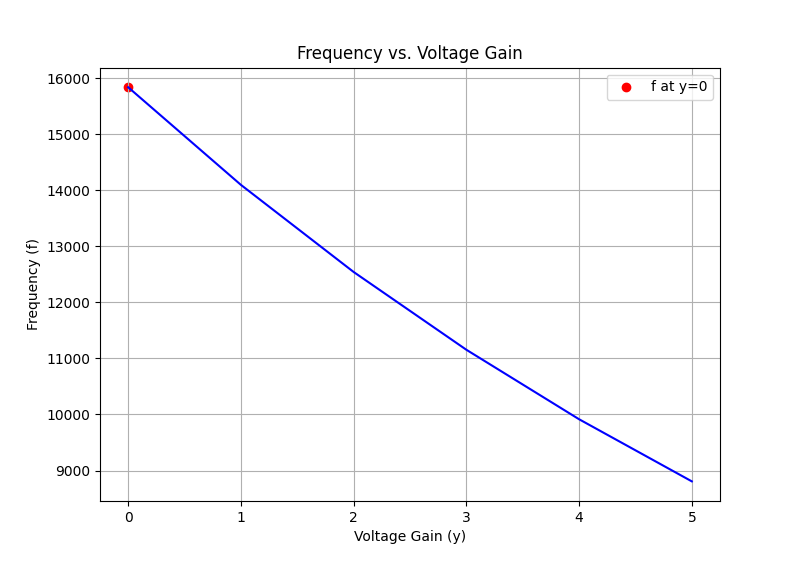
\includegraphics[width=\columnwidth]{figs/plot.png}
\label{fig:ttans_plott}
\caption{Frequency vs Voltage gain}
\end{figure}


\end{document}

